%%% Local Variables:
%%% mode: latex
%%% TeX-master: t
%%% End:

%%%%%%%%%%%%%%%%%%%% Preamble %%%%%%%%%%%%%%%%%%%%

\documentclass[11pt, paper=a4]{article}
\usepackage[utf8]{inputenc}

\usepackage[scale=0.8]{geometry}
\usepackage{amssymb,amsfonts,amsmath,latexsym,amsthm, mathtools} %mathtext,
\usepackage{booktabs}
\usepackage{multirow}
\usepackage{graphicx}
\usepackage{listings}
\usepackage{chngpage}
\usepackage{cprotect}
\usepackage{cite}
\usepackage{hyperref}
\usepackage{setspace}
\usepackage{parskip}


\graphicspath{{images/}}
\onehalfspacing{}

%%%%%%%%%%%%%%%%%%%% Document %%%%%%%%%%%%%%%%%%%%

\begin{document}

%%%%%%%%%%%%%%%%%%%% Title page %%%%%%%%%%%%%%%%%%%%

\title{{Report 2}\\{\bf Regression and Classification}}

\author{Markus Færevaag {\tt s123692} \& Jonathan Becktor {\tt s123094}}

\date{\today}

\maketitle

\begin{abstract}
  In this assignment we will explore Linear regression (LR), linear
  regression with forward selection (FLR), decision trees (DT), k
  nearest neighbors (KNN), naive bayes (NB), artificial neural networks
  (ANN), and multinomial regression (MNMR) methods.


  %% For regression
  %% problem, we found that the ANN model performs best, and the FLR and
  %% the average age (AVE) models are indistinguishable from each
  %% other. For classification problem, we found the ANN and MNMR to be the
  %% best performing models, and showed them to perform better than the
  %% largest class (LCl) classifier and the linear regression models (LR)
  %% using the paired t-test.
  %% Objective: The objective of this second report is to apply the
  %% methods you have learned in the second section of the course on
  %% ”Supervised learning: Classification and regression” in order to
  %% solve both a relevant classification and regression problem for your
  %% data.
\end{abstract}


%%%%%%%%%%%%%%%%%%%% Introduction %%%%%%%%%%%%%%%%%%%%
\section{Regression}
\label{sec:regression}
\subsection{Group issue}
Initially we were three people in our group. But due to our last group
member not finishing her part, and not letting us know that she would not
finish her part of the assignment, some of the answers will be
missing/lackluster. This is the second time she does not do
anything and now she no longer replies to our message. We have
therefore decided to remove her from our group.


\subsection{Problem description}
In this project the regession problem selected is to detect spam
emails from regular emails given 57 features.  The features used are
word-frequencies of 54 different words/signs, the amount of capital
letters, the longest sequence of capital letters and the average and
the average sequence of capital letters.

\subsection{Linear Regression with forward selection}
As the dataset has 57 features it is infeasable to compare them all
with LFR. Therefore for the for this section only the 12 first
features are used(in the figure only 6 features are compared). Firstly
the features are checked for any obvious relationships, and if it is
spam or not. From the figure~\ref{fig:modelcheck} it is hard to tell
if there is a distinct relationship between any of the features. If
any of them have a linear relationship they can be reduced to a single
feature. But this does reveal some patterns as you can see that almost
almost all of the emails that do not have the word our and have the
word 3d are spam.

\begin{figure}[h]
  \begin{minipage}{0.3\textwidth}
    a)\\
    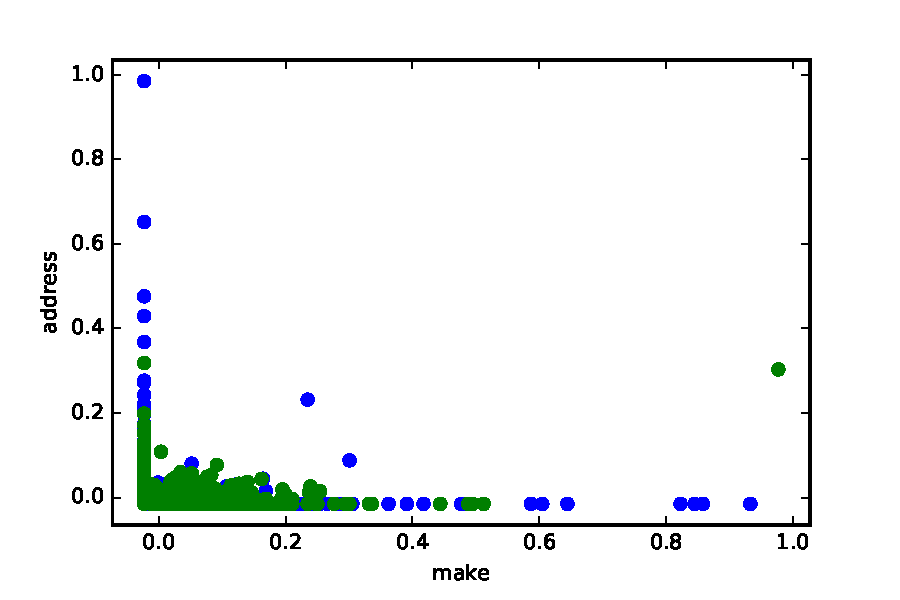
\includegraphics[width = 0.99\textwidth]{../../src/img/make_address.pdf}
  \end{minipage} \hfill
  \begin{minipage}{0.3\textwidth}
    b)\\
    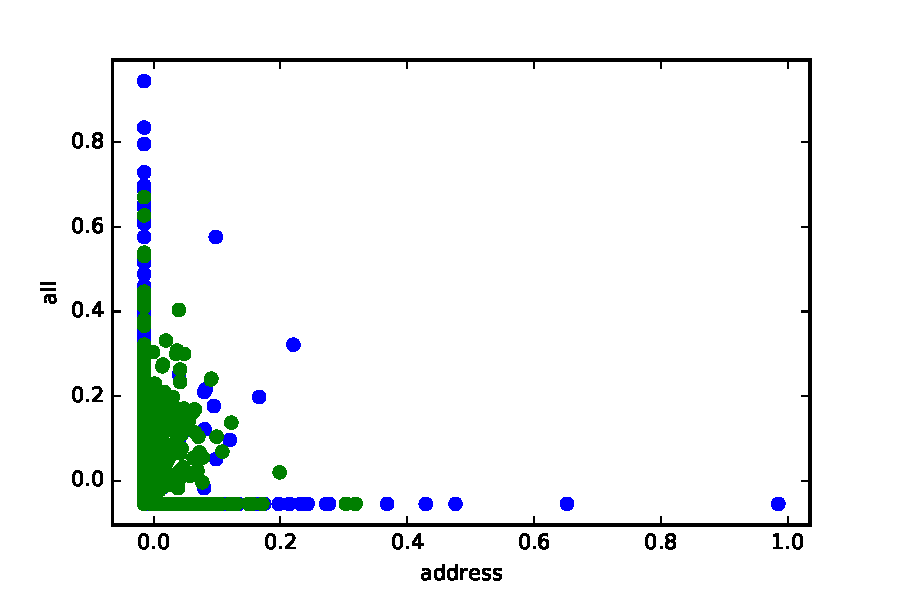
\includegraphics[width = 0.99\textwidth]{../../src/img/address_all.pdf}
  \end{minipage} \hfill
  \begin{minipage}{0.3\textwidth}
    c)\\
    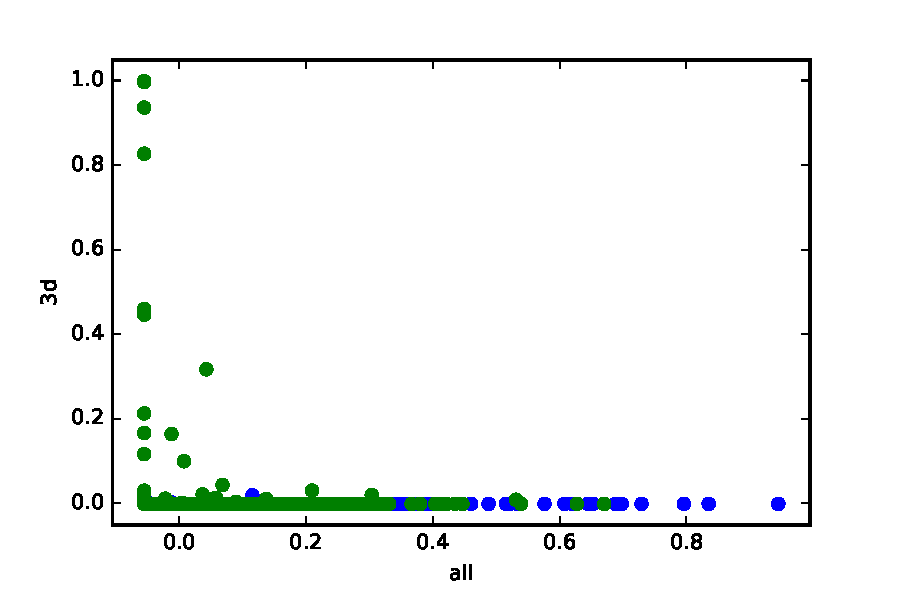
\includegraphics[width = 0.99\textwidth]{../../src/img/all_3d.pdf}
  \end{minipage} \vfill
  \begin{minipage}{0.3\textwidth}
    d)\\
    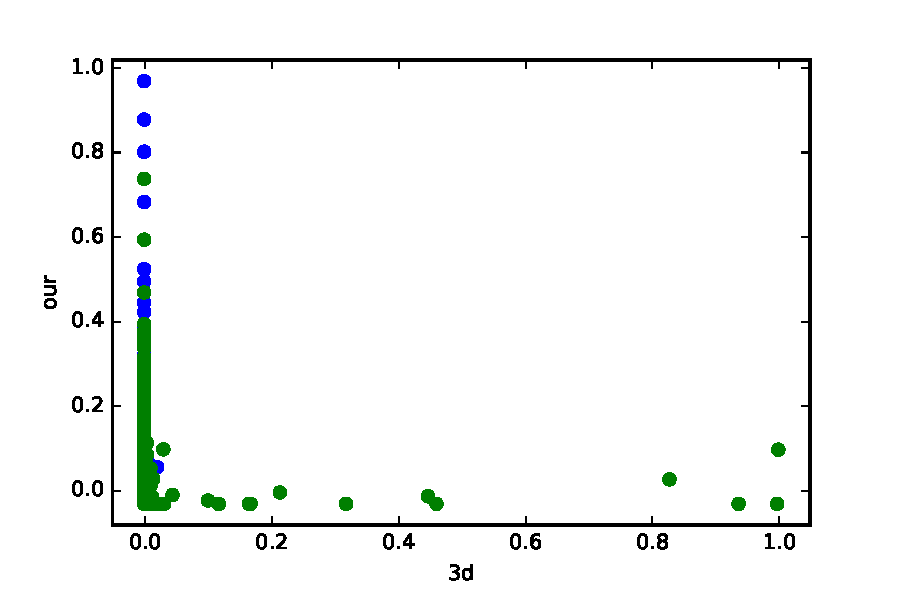
\includegraphics[width = 0.99\textwidth]{../../src/img/3d_our.pdf}
  \end{minipage} \hfill
  \begin{minipage}{0.3\textwidth}
    e)\\
    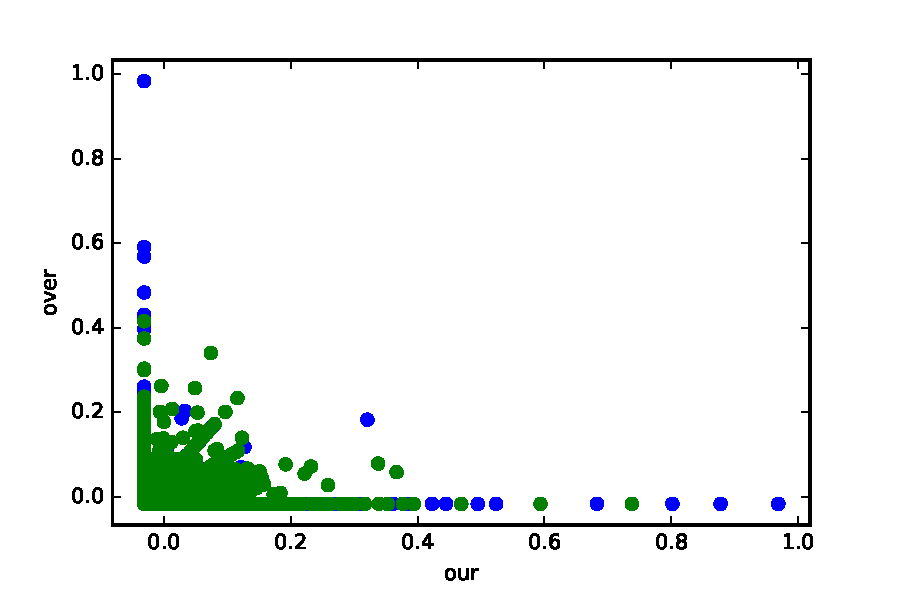
\includegraphics[width = 0.99\textwidth]{../../src/img/our_over.pdf}
  \end{minipage} \hfill
  \begin{minipage}{0.3\textwidth}
    f)\\
    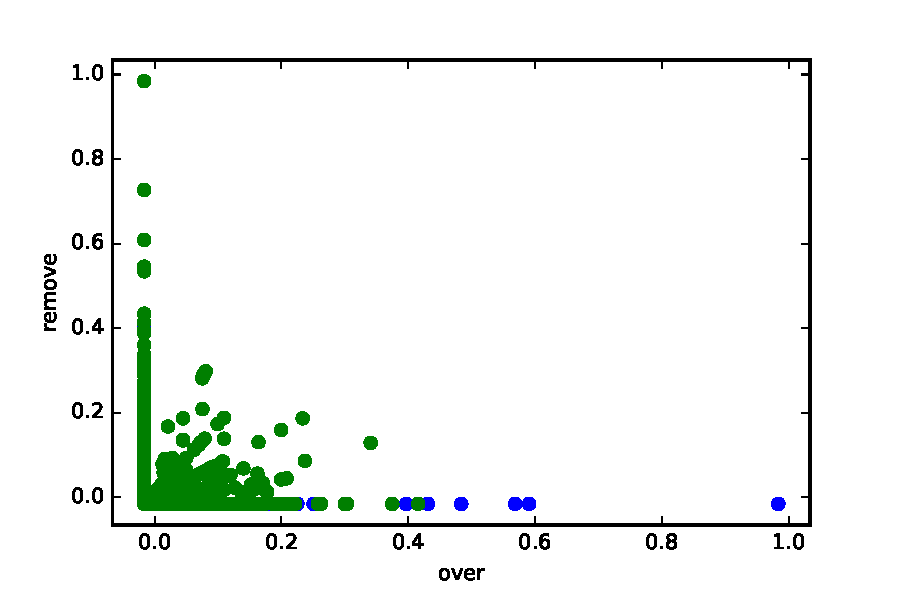
\includegraphics[width = 0.99\textwidth]{../../src/img/over_remove.pdf}
  \end{minipage} \vfill
  \caption{\label{fig:modelcheck} Green is spam and blue is not.}
\end{figure}

To figure out what features to use with LR we do forward selection
with a 10-fold cross-validation. Intially this would not run as the
initial loss with zero features had a lower error than any of the
features applied to it. Though to show that we forwar feature
selection on our dataset the inital loss was hardcoded
$loss\_record=[0.27]$.

\begin{figure}[h]
  \begin{minipage}{0.5\textwidth}
    a)\\
    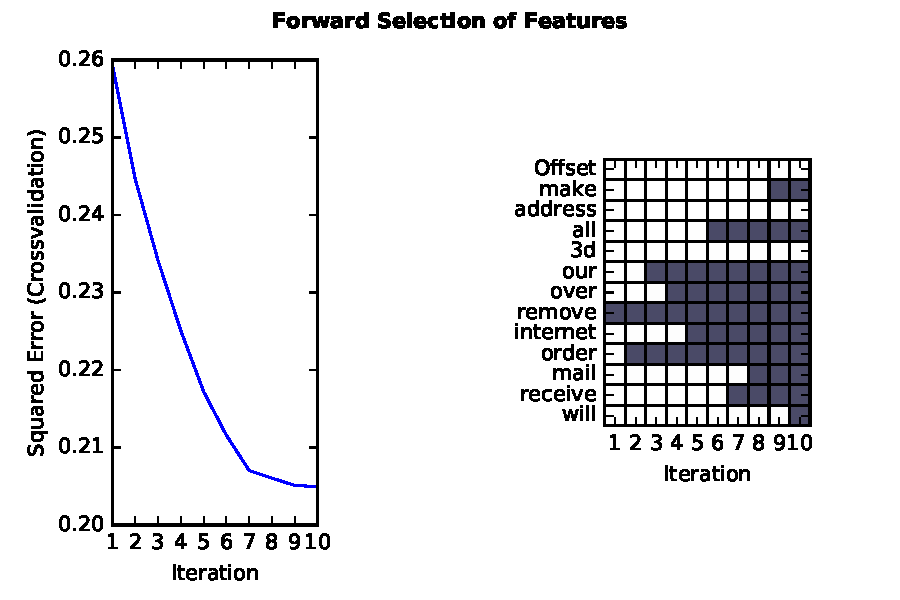
\includegraphics[width = 0.99\textwidth]{../../src/img/best_forward_selection.pdf}
  \end{minipage} \hfill
  \begin{minipage}{0.5\textwidth}
    b)\\
    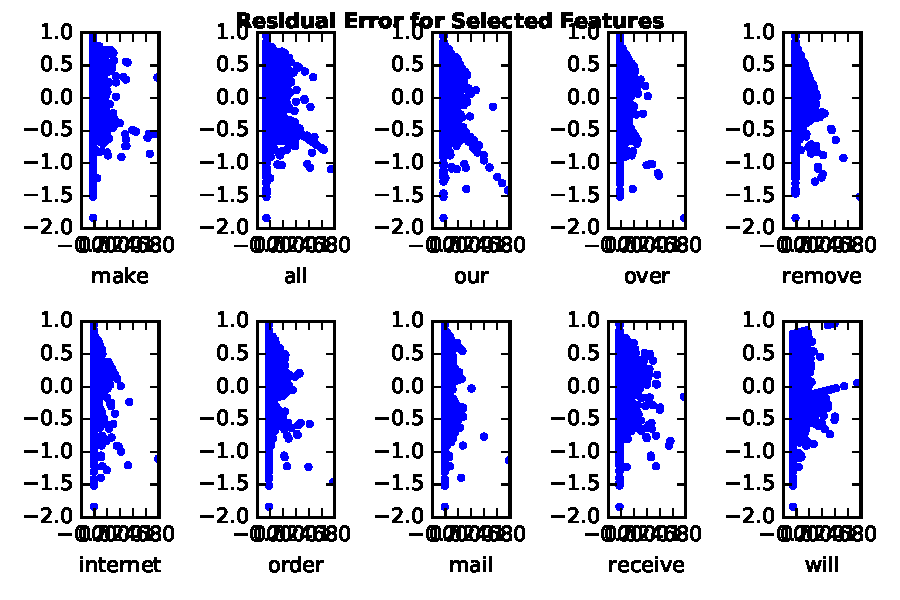
\includegraphics[width = 0.99\textwidth]{../../src/img/residual_error.pdf}
  \end{minipage} \hfill
  \caption{\label{fig:residual-error} Forward feature selection and
    Residual error for each feature. Note that the plot is slightly
    misleading as the spam is drawn on top of the nonspam and
    therefore it looks like there is much more spam}
\end{figure}

Above is the best feature selection that LRF could create with 12
features.  If we look at the error rates that are
computed:

\begin{figure}[h]
  \begin{minipage}{0.4\textwidth}
    \paragraph{Linear regression without feature selection:}
    \begin{itemize}
    \item Training error: 0.1673
    \item Test error:     0.1690
    \item $R^2$ train:     0.2993
    \item $R^2$ test:     0.2908
    \end{itemize}
  \end{minipage} \hfill
  \begin{minipage}{0.4\textwidth}
    \paragraph{Linear regression without feature selection:}
    \begin{itemize}
    \item Training error: 0.1681
    \item Test error:     0.1698
    \item $R^2$ train:     0.2985
    \item $R^2$ test:     0.2876
    \end{itemize}
  \end{minipage} \vfill
  \caption{Comparison of linear regression with and without feature selection}
\end{figure}
We can tell that without feature selection we get a smaller
error. Which leads us to believe that Linear Regression will not give
a great estimation of what is spam and what is not.

\subsection{Data predictions}
The fitted data has now created a model that can be used to fit the
email to spam or not.  The following vector are the coeficcients of
the trained model. These are the importance of each feature; which in
turn helps us estimate if an email is spam or not.

\begin{table}[h]
  \centering
  \begin{tabular}{c|c|c|c|c|c|c|c|c|c|c}
    \hline Attribute & make & all & our & over & remove & internet &
    order & mail & receive & will \\ \hline Coefficient & 0.490 &
    0.685 & 1.158 & 1.631 & 2.510 & 2.079 & 1.237 & 0.958 & 0.660 &
    -0.279 \\ \hline
  \end{tabular}
  \caption{Training model coefficients}
\end{table}

Above, in figure~\ref{fig:residual-error} the residual error for the different fearures can
be seen. From these we can conclued that something causes something
but they do not show any distinct patterns.

\subsection{Artificial Neural Network}
We implement an ANN model to try to solve the regression problem. Spam
is a binary variable as the mails can either be spam or not. The ANN
is implemented with $k=5$ cross-validation folds and $1-4$ hidden
units. Below in figure~\ref{fig:annhid} we have errorrates for the
fitted ANN's.  As can be seen from the figure we should use the ANN
with respectively 1 or 3 hidden units.


\begin{figure}[h]
  \centering
  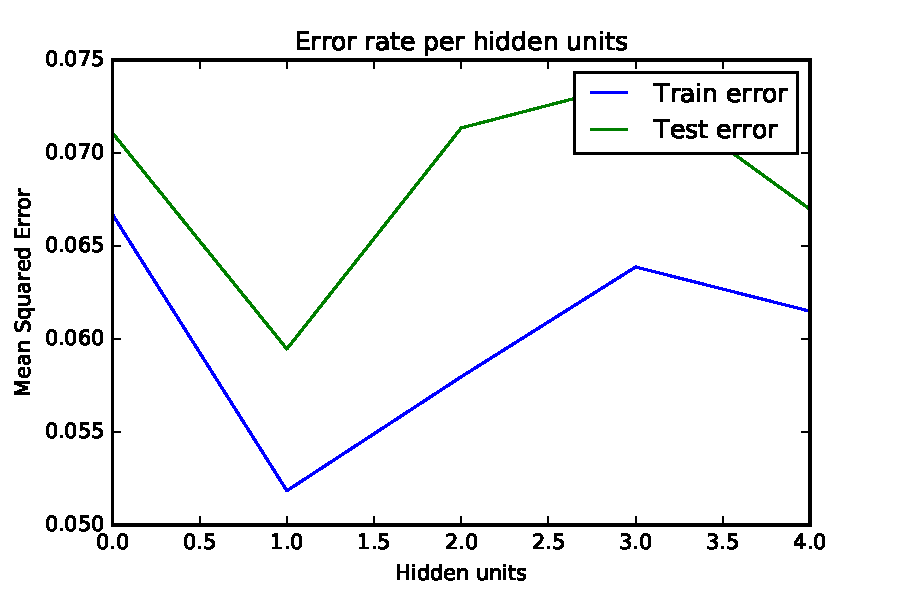
\includegraphics[width = 0.5\textwidth]{../../src/img/ann_regression_hid_units.pdf}
  \caption{Hidden units and error}
  \label{fig:annhid}
\end{figure}

\subsection{Model Comparison}
We now compare LRF with ANN. In figure~\ref{fig:compare} it is pretty
clear that the ANN results in a better error rate. Each of the ANN's
actually have better errorrates than LRF. Note that the comparison
only used a 5-k fold CV and only with 5 hidden units. This was done to
lower the running time of the network.

\begin{figure}[h]
  \begin{minipage}{0.5\textwidth}
    \paragraph{Artificial Neural Network w. (ANN):}
    \begin{itemize}
    \item Training error: 0.0534
    \item Test error:     0.0574
    \end{itemize}
  \end{minipage} \hfill
  \begin{minipage}{0.5\textwidth}
    \paragraph{Linear regression w. feature selection (LFR):}
    \begin{itemize}
    \item Training error: 0.16732
    \item Test error:     0.16908
    \end{itemize}
  \end{minipage} \vfill
  \caption{\label{fig:compare} Comparison between ANN and FLR}
\end{figure}


\clearpage
\section{Classification}

\subsection{Problem}
We have chosen to solve the classification using Decision Trees,
K-Nearest Neighbors and Naive Bayes, all using K-Fold cross-validation.

\subsection{Application}
From the three mentioned classification methods we get the following
error rates, using K-Fold cross-validation with $K=10$:
\begin{description}
  \item[Decision Tree] 7.54\%
  \item[Naive Bayes] 20.80\%
  \item[K-Nearest Neighbors] 20.54\%
\end{description}

In table~\ref{tbl:dt-feat} and~\ref{tbl:dt-nb}, we have ha comparison
of the five top features with the classification method producing the
lowest and highest error rate, respectively.

\begin{table}[h]
  \centering
  \begin{tabular}{c|c|c|c|c|c}
    \hline Attribute & {\tt \$} & {\tt remove} & {\tt !} & {\tt hp} & {\tt captial\_run\_length\_average} \\
    \hline Coefficient & 0.254 & 0.0131 & 0.108 & 0.069 & 0.063 \\
    \hline
  \end{tabular}
  \caption{\label{tbl:dt-feat} Top five features with Decision Tree}
\end{table}

\begin{table}[h]
  \centering
  \begin{tabular}{c|c|c|c|c|c}
    \hline Attribute & {\tt capital\_run\_length\_total} & {\tt *\_longest} & {\tt *\_average} & {\tt you} & {\tt your} \\
    \hline Coefficient & -0.237 & -1.734 & -4.132 & -5.550 & -6.043 \\
    \hline
  \end{tabular}
  \caption{\label{tbl:dt-nb} Top five features with Naive Bayes}
\end{table}

%%%%%%%%%%%%%%%%%%%% Bibliography %%%%%%%%%%%%%%%%%%%%
\clearpage

\end{document}
